\documentclass[a4paper,11pt]{article}
\usepackage{amsmath,amsthm,amsfonts,amssymb,amscd,amstext,vmargin,graphics,graphicx,tabularx,multicol} \usepackage[french]{babel}
\usepackage[utf8]{inputenc}  
\usepackage[T1]{fontenc} 
\usepackage[T1]{fontenc}
\usepackage{amsmath,amssymb}
\usepackage{pstricks-add,tikz,tkz-tab,variations}
\usepackage[autolanguage,np]{numprint} 

\setmarginsrb{1.5cm}{0.5cm}{1cm}{0.5cm}{0cm}{0cm}{0cm}{0cm} %Gauche, haut, droite, haut
\newcounter{numexo}
\newcommand{\exo}[1]{\stepcounter{numexo}\noindent{\bf Exercice~\thenumexo} : \marginpar{\hfill /#1}}
\reversemarginpar


\newcounter{enumtabi}
\newcounter{enumtaba}
\newcommand{\q}{\stepcounter{enumtabi} \theenumtabi.  }
\newcommand{\qa}{\stepcounter{enumtaba} (\alph{enumtaba}) }
\newcommand{\initq}{\setcounter{enumtabi}{0}}
\newcommand{\initqa}{\setcounter{enumtaba}{0}}

\newcommand{\be}{\begin{enumerate}}
\newcommand{\ee}{\end{enumerate}}
\newcommand{\bi}{\begin{itemize}}
\newcommand{\ei}{\end{itemize}}
\newcommand{\bp}{\begin{pspicture*}}
\newcommand{\ep}{\end{pspicture*}}
\newcommand{\bt}{\begin{tabular}}
\newcommand{\et}{\end{tabular}}
\renewcommand{\tabularxcolumn}[1]{>{\centering}m{#1}} %(colonne m{} centrée, au lieu de p par défault) 
\newcommand{\tnl}{\tabularnewline}

\newcommand{\trait}{\noindent \rule{\linewidth}{0.2mm}}
\newcommand{\hs}[1]{\hspace{#1}}
\newcommand{\vs}[1]{\vspace{#1}}

\newcommand{\N}{\mathbb{N}}
\newcommand{\Z}{\mathbb{Z}}
\newcommand{\R}{\mathbb{R}}
\newcommand{\C}{\mathbb{C}}
\newcommand{\Dcal}{\mathcal{D}}
\newcommand{\Ccal}{\mathcal{C}}
\newcommand{\mc}{\mathcal}

\newcommand{\vect}[1]{\overrightarrow{#1}}
\newcommand{\ds}{\displaystyle}
\newcommand{\eq}{\quad \Leftrightarrow \quad}
\newcommand{\vecti}{\vec{\imath}}
\newcommand{\vectj}{\vec{\jmath}}
\newcommand{\Oij}{(O;\vec{\imath}, \vec{\jmath})}
\newcommand{\OIJ}{(O;I,J)}

\newcommand{\bmul}[1]{\begin{multicols}{#1}}
\newcommand{\emul}{\end{multicols}}


\newcommand{\reponse}[1][1]{%
\multido{}{#1}{\makebox[\linewidth]{\rule[0pt]{0pt}{20pt}\dotfill}
}}

\newcommand{\titre}[5] 
% #1: titre #2: haut gauche #3: bas gauche #4: haut droite #5: bas droite
{
\noindent #2 \hfill #4 \\
#3 \hfill #5

\vspace{-1.6cm}

\begin{center}\rule{6cm}{0.5mm}\end{center}
\vspace{0.2cm}
\begin{center}{\large{\textbf{#1}}}\end{center}
\begin{center}\rule{6cm}{0.5mm}\end{center}
}



\begin{document}
\pagestyle{empty}
\titre{Contrôle : Nombres relatifs, périmètres et aires}{Nom :}{Prénom :}{Classe}{Date}

\begin{tabular}{|m{11cm}|c|c|c|}
\hline 
\textbf{Compétences} & \textbf{Acquis} & \textbf{En cours}  & \textbf{Non acquis} \\ 
\hline 
- Connaître la notion de nombre opposé. &  &  & \\
\hline
- Savoir ranger et comparer des nombres relatifs. &  &  &  \\ 
\hline 
- Savoir calculer le périmètre d'une figure et l'exprimer dans la bonne unité. &  &  &  \\ 
\hline 
- Savoir calculer l'aire d'une surface simple et l'exprimer dans la bonne unité. &  &  &  \\ 
\hline 
- Savoir calculer l'aire d'une surface par décomposition en surfaces dont les aires sont facilement calculables et l'exprimer dans la bonne unité.  &  &  &  \\ 
\hline 


\end{tabular} 


\vspace*{1cm}

\exo{3} Ranger ces évènements du plus anciens au plus récents.

\bmul{3}

\textbf{- 300} :	Bérose, un astronome, invente le cadran solaire vertical. \\

\textbf{105} :	Les chinois invente le papier. \\

\textbf{- 212} :	Mort d'Archimède. \\


\columnbreak

\textbf{- 330} : 	Naissance d'Euclide.\\

 \textbf{ 498} :	L'indien Ardjabatta explique le mécanisme des éclipses.\\ 
  
\textbf{- 59 }:	 César envahit la Gaule.\\


\columnbreak


\textbf{- 490} :	Bataille de Marathon.\\

  \textbf{326} : 	Fondation de Constantinople. \\
  
\textbf{- 30} : 	Mort de Cléopâtre.\\


\emul

\vspace*{1cm}

\exo{2}Dire si les affirmations sont vraies ou fausses. Aucune justification n'est demandée.\\

\initq \q L'opposé d'un nombre est toujours un nombre négatif.\\

\q Deux nombres opposés non nuls sont de signes contraires.\\

\q Un nombre positif est plus grand qu'un nombre négatif.\\

\q Un nombre négatif est un nombre inférieur à 0.\\



\vspace*{1cm}

\exo{3.5} Calculer le périmètre des figures suivantes :\\


\bmul{3}


\initqa \qa 

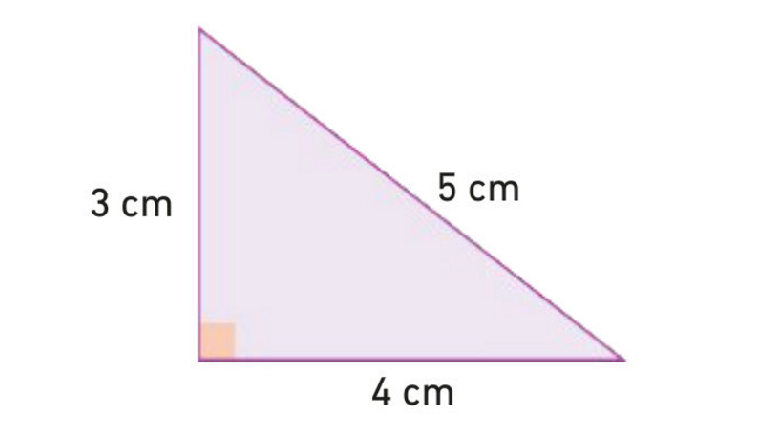
\includegraphics[scale=0.4]{perim1.eps} \\



\columnbreak


\qa 

 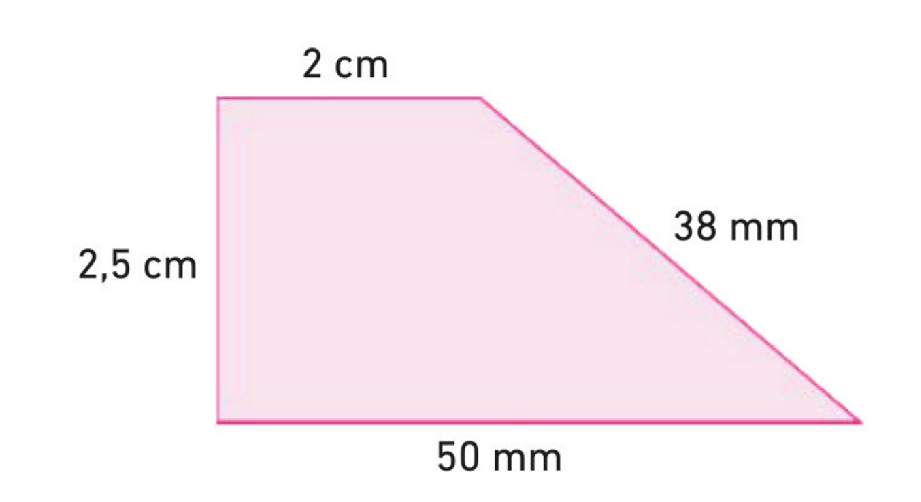
\includegraphics[scale=0.4]{perm2.eps} \\


\columnbreak


\qa 

 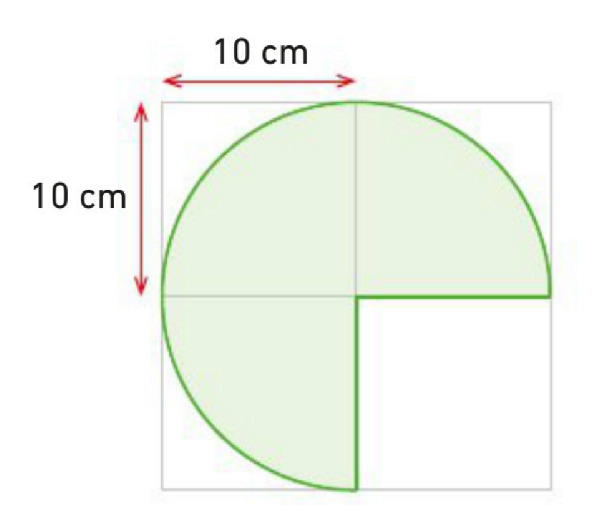
\includegraphics[scale=0.4]{perim3.eps} \\


\emul

\newpage

\exo{2.5}\\
Sachant que le côté d'un carreau mesure 1cm, déterminer l'aire des figures suivantes :\\

\begin{center}
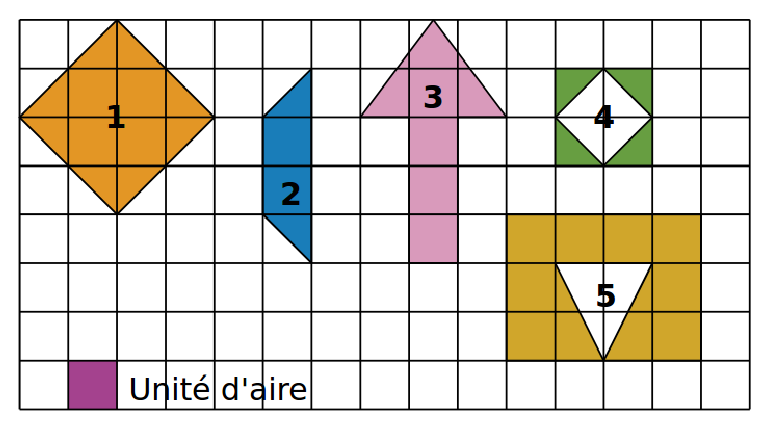
\includegraphics[scale=0.75]{exoaire.eps} 
\end{center}


\vspace*{0.5cm}

\exo{4}
Calculer l'aire des figures suivantes. Donner la réponse en $mm^{2}$.


\bmul{2}

\initqa \qa 

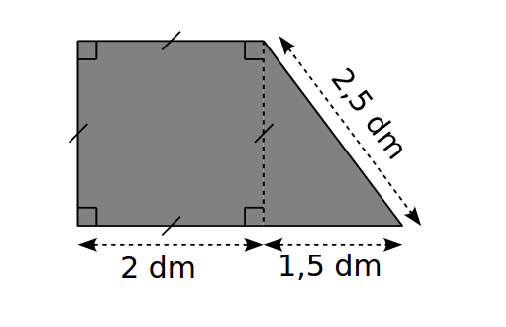
\includegraphics[scale=0.8]{exoaires2.eps} 

\columnbreak

\qa 

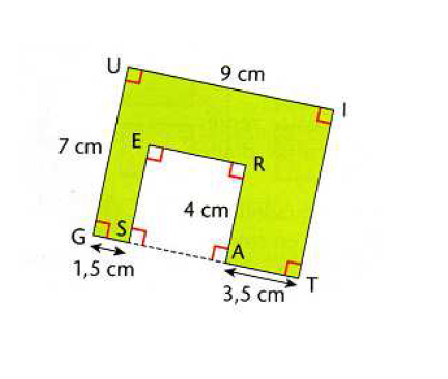
\includegraphics[scale=0.9]{aires1.eps} 

\emul








\vspace*{0.5cm}

\exo{3}\\

\initq \q Calculer l'aire d'un disque de diamètre 20 m.\\

\q Un rectangle a une longueur de 2,5 cm et une aire de 12.5 $cm^{2}$. Calculer sa largeur.\\

\vspace*{0.5cm}

\exo{2}\\
 Le rectangle et le carré ci-dessous ont le même périmètre.
Calculer l'aire du carré.

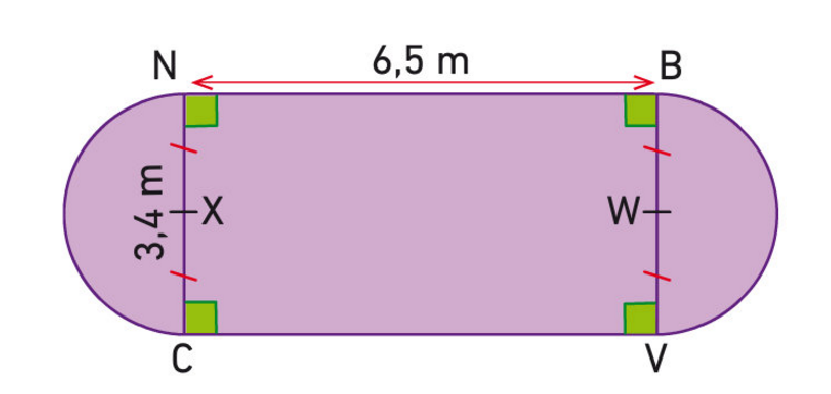
\includegraphics[scale=1]{aires3.eps} \\





\vspace*{0.5cm}




\exo{} BONUS\\

Je suis un rectangle dont les côtés mesurent un nombre entier de centimètres. Mon aire est égale a 120 $cm^{2}$ et mon périmètre est égal à 52 cm. \\
Quelles sont mes dimensions ?\\



\end{document}
